\switchcolumn[1]*
\codeblock{kfac/scaffold}
\switchcolumn[0]

KFAC has many nuances that complicate its understanding.
However, we can break down its structure into a general scaffold that simplifies its complexity into manageable sub-tasks (\Cref{kfac/scaffold}).
Here, we discuss the components.

\paragraph{Outline.} At its core, KFAC approximates curvature matrices using Kronecker products, significantly reducing computational and memory costs.
In this section, we start from the general form of relevant curvature matrices, discuss how their structure enables a Kronecker-factored approximation, and introduce the core components of KFAC.
This scaffold---accompanied by the code snippets on the right---serves as the foundation for a systematic implementation, offering intuition on how Kronecker factors are computed and why such a decomposition is beneficial.
We keep the discussion general and highlight how to adapt the code to approximate any curvature matrix introduced in the previous section.
The next section (\Cref{sec:kfac-expand-linear}) will focus on the specific case of KFAC for the generalized Gauss-Newton (GGN) of linear layers.

\paragraph{Curvature matrix structure.} Many relevant matrices---like the GGN, the type-I, type-II, and empirical Fisher---share a common structure
\begin{align}\label{eq:common-structure}
  \begin{split}
    \!\!\mC&(\vtheta^{(i)}) \\
           &= R \sum_n
             (\jac_{\vtheta^{(i)}} \vf_n)^{\top}
             \left[ \bullet(\vf_n, \vy_n) \right]
             (\jac_{\vtheta^{(i)}} \vf_n)\,
  \end{split}
\end{align}
where $\bullet \in \sR^{\dim(\gF) \times \dim(\gF)}$ is a positive semi-definite matrix in the prediction space that depends on the prediction $\vf_n$ and target $\vy_n$.
This term is sandwiched between the Jacobians of the network's prediction with respect to the parameters $\vtheta^{(i)}$ in layer $i$.
Directly computing and storing these matrices is usually intractable, which motivates approximation schemes such as KFAC.
\paragraph{Key idea.} The idea behind KFAC is to exploit a Kronecker-product structure in the Jacobians $\jac_{\vtheta^{(i)}}\vf_n$ to approximate
\begin{align*}
  \mC(\vtheta^{(i)})
  \approx
  \kfac(\mC(\vtheta^{(i)}))
  \coloneqq \mA^{(i)} \otimes \mB^{(i)}.
\end{align*}
For a composition of functions $$f \coloneqq f^{(L)} \circ f^{(L-1)} \circ \dots \circ f^{(1)}$$ with parameters $$\vtheta = \left[ \vtheta^{(1)}, \dots, \vtheta^{(L)} \right],$$ KFAC yields a block-diagonal approximation of the full curvature matrix $\mC(\vtheta)$, where each block corresponds to a layer and is of the form $\kfac(\mC(\vtheta^{(i)})) = \mA^{{(i)}} \otimes \mB^{(i)}$.

In this approximation, $\mA^{(i)}$ is computed from the inputs to layer $i$, and we refer to it as \emph{input-based Kronecker factor}.
Similarly, $\mB^{(i)}$ is computed from gradients \wrt layer $i$'s output, and we call it the \emph{grad-output-based Kronecker factor}.

\subsection{Why use a Kronecker structure?}
Having a Kronecker approximation for $\mC(\vtheta^{(i)})$ has multiple advantages and motivations, that coincide well with the block diagonal structure.

\subsubsection{Kronecker Products Are Computationally Efficient}
\label{sec:mem_comp_eff_kron}
Instead of working with the dense representation
\begin{align*} \mA \otimes& \mB  \in \R^{n_1m_1 \times n_2m_2} \\
                          &=\begin{bmatrix}
                            a_{1,1} & \dots & a_{1,n_2} \\
                            \vdots & \ddots & \vdots \\
                            a_{n_1,1} & \dots & a_{n_1,n_2}
                          \end{bmatrix}
  \\
                          &\otimes
                            \begin{bmatrix}
                              b_{1,1} & \dots & b_{1,m_2} \\
                              \vdots & \ddots & \vdots \\
                              b_{m_1,1} &  \dots & b_{m_1,m_2}
                            \end{bmatrix} \\
                          &=\begin{bmatrix}
                            a_{1,1} \mB & \dots & a_{1,n_2} \mB \\
                            \vdots & \ddots & \vdots \\
                            a_{n_1,1} \mB & \dots & a_{n_1,n_2} \mB
                          \end{bmatrix}\,,
\end{align*}
we can express many operations with the Kronecker factors $\mA \in \sR^{n_1 \times n_2}$ and $\mB \in \sR^{m_1 \times m_2}$.
This drastically reduces memory, as we only need to store and handle these smaller matrices (\ie, $\mathcal{O}(n_1n_2 + m_1m_2)$) rather than the full Kronecker product (\ie $\mathcal{O}(n_1n_2m_1m_2)$).
Examples are:

\paragraph{Matrix-vector products.}
Let $\vv \in \R^{n_2m_2}$, then
$$ (\mA \otimes \mB) \vv = \cvec(\mB \mV \mA^{\top}) $$
with $\mV = \cvec^{-1}(\vv) \in \R^{n_2\times m_2}$.
Similarly,
$$ (\mA \otimes \mB) \vv = \rvec(\mA \mV \mB^{\top}) $$
with $\mV = \rvec^{-1}(\vv) \in \R^{m_2\times n_2}$.

\paragraph{Matrix transpose.} $(\mA \otimes \mB)^{\top} = \mA^{\top} \otimes \mB^{\top}$.

\paragraph{Matrix inverse.} $(\mA \otimes \mB)^{-1} = \mA^{-1} \otimes \mB^{-1}$ (assuming the Kronecker factors are invertible).

\paragraph{Matrix multiplication.}
Let $\mC \in \R^{n_2 \times d_1}$ and $\mD \in \R^{m_2 \times d_2}$, then we have
$$ (\mA \otimes \mB)(\mC \otimes \mD) = \mA \mC \otimes \mB \mD\,, $$ \ie we can multiply the Kronecker factors.

\subsubsection{Kronecker Products Naturally Emerge in Curvature Matrices}

Kronecker structure arises naturally in the expression for $\mC(\vtheta^{(i)})$ due to the structure of the layer Jacobians, providing a strong motivation for its use.
To see this, we rewrite $\mC(\vtheta^{(i)})$ from \Cref{eq:common-structure}.

\paragraph{Factorizing the loss Hessian.}
Since $\bullet(\vf_n, \vy_n)$ is a positive semi-definite matrix, it can be decomposed as a sum of outer products of at most $\dim(\gF)$ vectors: $$\bullet(\vf_n, \vy_n) = \sum_{c=1}^{\dim(\gF)} \blacktriangle_c(\vf_n, \vy_n) (\blacktriangle_c(\vf_n, \vy_n))^{\top}$$
where we define $\blacktriangle_{n,c} := \blacktriangle_c(\vf_n, \vy_n) \in \sR^{\dim(\gF)}$ as a vector we will specify later.
Substituting this into \Cref{eq:common-structure}, we obtain
\begin{align*}
  \mC(&\vtheta^{(i)}) \\
  =&
     R \sum_n \sum_{c}
     (\jac_{\vtheta^{(i)}} \vf_n)^{\top}
     \blacktriangle_{n,c} \blacktriangle_{n,c}^{\top}
     (\jac_{\vtheta^{(i)}} \vf_n)\,.
\end{align*}

\paragraph{Separate the layer's Jacobian.}
By applying the chain rule to split the Jacobian at the layer output $\vx^{(i)} = f^{(i)}(\vx^{(i-1)}, \vtheta^{(i)})$, we get
\begin{align*}
  (\jac_{\vtheta^{(i)}} \vf_n)^{\top}
  =
  (\jac_{\vtheta^{(i)}} \vx^{(i)}_n)^{\top}
  (\jac_{\vx_n^{(i)}} \vf_n)^{\top}.
\end{align*}
Substituting this back, the curvature matrix is
\begin{align*}
  \mC(\vtheta&^{(i)}) \\ =& R \sum_n \sum_{c}
                          &&(\jac_{\vtheta^{(i)}} \vx^{(i)}_n)^{\top} \\
             & &&(\jac_{\vx_n^{(i)}} \vf_n)^{\top}
                  \blacktriangle_{n,c}
                  \blacktriangle_{n,c}^{\top}
                  (\jac_{\vx_n^{(i)}} \vf_n) \\
             & &&(\jac_{\vtheta^{(i)}} \vx^{(i)}_n).
\end{align*}

\paragraph{Insert the layer's Jacobian.}
The Kronecker structure emerges naturally in the output-parameter Jacobian $\jac_{\vtheta^{(i)}} \vx_n^{(i)}$ of a layer.
We saw this in previous chapters for a linear layer (\Cref{ex:linear_layer_jacobians}), whose Jacobian is a Kronecker product of the layer input $\vx^{(i-1)}_n$ and an identity matrix.
Without showing the explicit expression when inserting a Jacobian (this will be part of the next chapter), we note that this reduces the \emph{exact} form of $\mC^{(i)}$ to a sum of Kronecker products.
\begin{align*}
  \mC^{(i)} = R \sum_n \sum_c \va_n \va_n^{\top} \otimes \vb_{n,c} \vb_{n,c}^{\top}
\end{align*}
where $\va_n$ stems from the layer's Jacobian, \ie the layer's input, and $\vb_{n,c}$ stems from the vector $\blacktriangle_{n,c}$ that is backpropagated to the layer's output by applying the Jacobian $(\jac_{\vx_n^{(i)}} \vf_n)^{\top}$.

Our remaining steps are (i) to specify what $\va_n$ and $\vb_{n,c}$ are, which will depend on the curvature matrix we want to approximate (\Cref{subsec:backpropagated-vectors}), and (ii) how to approximate the sum of Kronecker products as a single Kronecker product (KFAC's expectation approximation, \Cref{def:kfac_exp_approx}).

\switchcolumn[1]*
\codeblock{kfac/backpropagated_vectors}
\switchcolumn[0]

\subsubsection{Kronecker Factor Dependencies}

For the scaffold in \Cref{kfac/scaffold}, let's quickly think about the dependencies of the Kronecker matrices in the above expression.
KFAC results in two distinct Kronecker factors: one based on layer inputs (input-based Kronecker factor $\mA^{(i)}$) and the other based on gradients with respect to the layer output (grad-output-based Kronecker factor $\mB^{(i)}$).
As we will see, we can interpret $(\jac_{\vtheta^{(i)}} \vx_n^{(i)})^{\top} \blacktriangle_{n,c}$ as a \emph{pseudo-gradient}.
In fact, setting
$$\blacktriangle_{n,c} \leftarrow \nabla_{\vf_n} c(\vf_n, \vy_n)\,$$
we obtain
$$(\jac_{\vtheta^{(i)}} \vx_n^{(i)})^{\top} \blacktriangle_{n,c} = \nabla_{\vx_n^{(i)}} c(\vf_n, \vy_n),$$
which is the per-datum loss gradient with respect to layer $i$'s output.
In summary, we identify the following dependencies of the Kronecker factors $\mA^{(i)}$ and $\mB^{(i)}$, justifying their names:
\begin{align*}
  \mA^{(i)} &\text{\quad depends on \quad} \{\vx_{n}^{(i-1)}\}_n \,,
  \\
  \mB^{(i)} &\text{\quad depends on \quad} \{ (\jac_{\vx_n^{(i)}}\vf_{n})^{\top} \blacktriangle_{n,c}\}_{n,c}\,.
\end{align*}

\subsection{Algorithmic Outline}

We now know enough to discuss the scaffold from \Cref{kfac/scaffold}.

\paragraph{Step 1:} Perform a forward pass to compute $\{\vf_n\}_n $, storing the layer inputs $\{\vx_n^{(i-1)} \}_n$ and outputs $\{\vx_n^{(i)}\}_n$ of all layers $i$ whose parameter curvature matrix we want to approximate with KFAC.

\paragraph{Step 2:} Compute the input-based Kronecker factors $\mA^{(i)}$ using the layer inputs $\{\vx_n^{(i-1)}\}_n$.
The details of that will depend on the layer type and we still have to specify them in later chapters.

\paragraph{Step 3:} Generate the vectors $\{\blacktriangle_{n,c}\}_{n,c}$ to be backpropagated, and backpropagate them to the layer outputs to get the pseudo-gradients $\{(\jac_{\vx_n^{(i)}} \vf_n)^{\top} \blacktriangle_{n,c} \}_{n,c}$.
This step depends on the loss function we are using, and the curvature matrix we want to approximate (\Cref{subsec:backpropagated-vectors}).
Finally, compute the output-based Kronecker factors $\mB^{(i)}$.
The details will again depend on the layer type and we will specify them in later chapters.

\paragraph{Step 4:} Account for scaling caused by the loss function's reduction $R$.

\paragraph{Step 5:} Return the KFAC approximation in the form $\mA^{(i)}, \mB^{(i)}$ for all supported $i$.

In summary, the scaffold disentangles the task of computing KFAC into three components: (i) computing the input-based Kronecker factors, (ii) generating and backpropagating the vectors $\blacktriangle_{n,c}$, and (iii) computing the grad-output-based Kronecker factors.
The next section describes how to accomplish step (ii).
After that, we can add new KFAC implementations simply by specifying (i) and (iii) for each new layer.

\subsection{Backpropagated Vectors}\label{subsec:backpropagated-vectors}
The computational scaffold can be flexibly adapted to various curvature matrices by modifying the choice of backpropageted vectors $\blacktriangle_{n,c}$ and the reduction factor $R$.
This can be done by pattern-matching each curvature matrix to the general form in \Cref{eq:common-structure}.
Below, we recap the different curvature definitions; see \Cref{subsec:curvature-matrices} for a self-contained introduction.

\paragraph{Generalized Gauss-Newton/type-II Fisher.} Remember the GGN from \Cref{sec:partial_linearization},
\begin{align*}
  \mG(\vtheta)= R \sum_n
  \left[\jac_{\vtheta} \vf_n\right]^{\top}
  \left[\hess_{\vf_n} c(\vf_n, \vy_n)
  \right]
  \left[\jac_{\vtheta} \vf_n\right]\,.
\end{align*}
Using the symmetric decomposition
$$\mS_n \mS_n^{\top} = \hess_{\vf_n} c(\vf_n, \vy_n),$$ we identify for the backprograted vector
\begin{align*}
  \blacktriangle_{n,c} = [\mS_n]_{:,c}.
\end{align*}
In words, to approximate the GGN with KFAC, we must backpropagate each of the $\dim(\gF)$ columns of the Hessian decomposition $\mS_n$.
For common loss functions, the Type-II Fisher from \Cref{sec:fisher} coincides with the GGN, hence we can use the same backpropagated vectors as for the GGN to approximate it.

\paragraph{MC-sampled type-I Fisher.}
The type-I Fisher, approximated via Monte Carlo (MC) sampling, is
\begin{align*}
  &\begin{aligned}
    \mF^{\text{I}}(\vtheta) = \lim_{M \to \infty} \frac{R}{M} \sum_{n=1}^N
    &\left( \jac_{\vtheta} \vf_n\right)^{\top} \\
    &
      \begin{aligned}
        \big[
        &\nabla_{\vf_n} c(\vf_n, \tilde{\vy}_{n,m}) \\
        &\nabla_{\vf_n} c(\vf_n, \tilde{\vy}_{n,m})^{\top}
          \big]
      \end{aligned} \\
    &\jac_{\vtheta} \vf_n\,,
  \end{aligned}
\end{align*}
(\Cref{sec:fisher}).
We can immediately see that
\begin{align*}
  \blacktriangle_{n,m}
  &= \nabla_{\vf_n}  c(\vf_n, \tilde{\vy}_{n,m})
\end{align*}
where $\tilde{\vy}_{n,m} \stackrel{\text{\iid}}{\sim} r(\rvy \mid \vf = \vf_n)$ is a sample from the model's predictive distribution.
In words, to approximate the Type-I Fisher with KFAC, we backpropagate $M$ `would-be' gradients for each datum $\vf_n$.
The number of Monte Carlo samples controls the number of backpropagations:
\begin{itemize}
\item For \emph{computational efficiency}, $M<\dim(\gF)$ makes sense because this reduces the number of backpropagations from $\dim(\gF)$ (as in the type-II case) to $M$.
\item For \emph{practical settings} $M$ is usually set to $1$.
\item For \emph{verification}, a larger $M$ can be used to ensure convergence to the expected value.
\end{itemize}

\paragraph{Empirical Fisher.}
The empirical Fisher (\Cref{sec:emp_fisher}) replaces the expectation over the model's likelihood in the type-I Fisher by the expectation over the empirical distribution:
\begin{align*}
  &\begin{aligned}\mE(\vtheta) = R \sum_{n=1}^N
    &\jac_{\vtheta} \vf_n^{\top} \\
                               & \nabla_{\vf_n} c(\vf_n, \tilde{\vy}_{n}) (\nabla_{\vf_n} c(\vf_n, \tilde{\vy}_n ))^{\top} \\
                               &\jac_{\vtheta} \vf_n\,.
  \end{aligned}
\end{align*}
We identify that we only need to backpropagate a single vector per datum,
\begin{align*}
  \blacktriangle_{n,1}
  &= \nabla_{\vf_n}  c(\vf_n, \vy_n)\,.
\end{align*}
It is the same vector that is backpropagated to compute the gradient.
This means that to approximate the empirical Fisher with KFAC, we can re-cycle the backward pass from the gradient computation.

\switchcolumn[1]*
\begin{figure}[t!]
  \centering
  \begin{minipage}[t]{0.485\linewidth}
    \centering
    \textbf{FULL}
  \end{minipage}
  \hfill
  \begin{minipage}[t]{0.485\linewidth}
    \centering
    \textbf{KFAC}
  \end{minipage}
  \\
  \begin{minipage}[t]{0.485\linewidth}
    \centering
    GGN ($\cvec$)\vspace{1ex}
    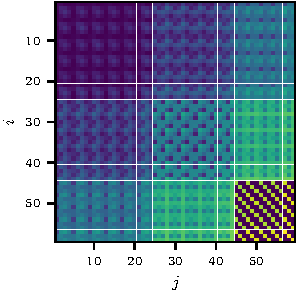
\includegraphics[width=0.8\linewidth]{../kfs/plots/synthetic_cvec_ggn_full.pdf}
  \end{minipage}
  \hfill
  \begin{minipage}[t]{0.485\linewidth}
    \centering
    GGN ($\cvec$)\vspace{1ex}
    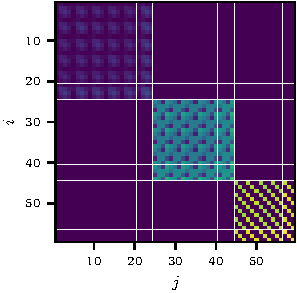
\includegraphics[width=0.8\linewidth]{../kfs/plots/synthetic_cvec_ggn_kfac.pdf}
  \end{minipage}
  \\
  \begin{minipage}[t]{0.485\linewidth}
    \centering
    MC-Fisher ($\cvec$)\vspace{1ex}
    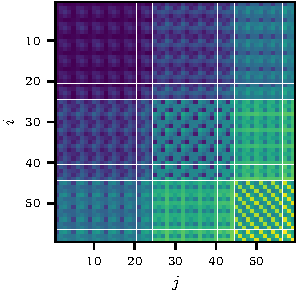
\includegraphics[width=0.8\linewidth]{../kfs/plots/synthetic_cvec_mcfisher_100_full.pdf}
  \end{minipage}
  \hfill
  \begin{minipage}[t]{0.485\linewidth}
    \centering
    MC-Fisher ($\cvec$)\vspace{1ex}
    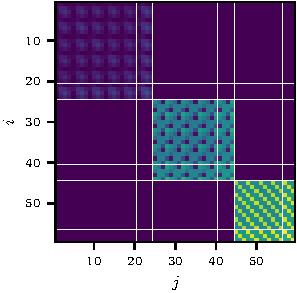
\includegraphics[width=0.8\linewidth]{../kfs/plots/synthetic_cvec_mcfisher_100_kfac.pdf}
  \end{minipage}
  \\
  \begin{minipage}[t]{0.485\linewidth}
    \centering
    Emp-Fisher ($\cvec$)\vspace{1ex}
    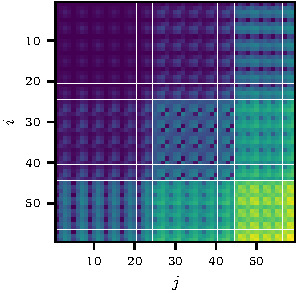
\includegraphics[width=0.8\linewidth]{../kfs/plots/synthetic_cvec_empfisher_full.pdf}
  \end{minipage}
  \hfill
  \begin{minipage}[t]{0.485\linewidth}
    \centering
    Emp-Fisher ($\cvec$)\vspace{1ex}
    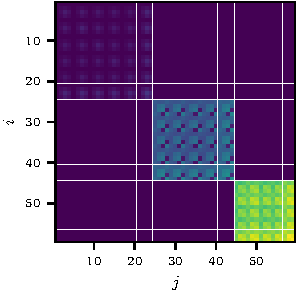
\includegraphics[width=0.8\linewidth]{../kfs/plots/synthetic_cvec_empfisher_kfac.pdf}
  \end{minipage}
  \caption{Visualization of full curvatures (GGN, MC-sampled Fisher and Empirical Fisher) and their corresponding KFAC approximation using $\cvec$-flattening. All curvatures were evaluated on synthetic data ($N = 100$) using an MLP with three fully-connected layers and ReLU activations (5-4-4-3, our notation considers applying the weight matrix and adding the bias as two layers, hence $L=6$) and square loss. For the MC-sampled Fisher we consider $M = 100$ Monte Carlo samples. This follows the setup in \Cref{fig:hessian-block-structure}. For KFAC we concatenate the weight and bias of each layer.
    Plots produced with \repofile{plots/synthetic_kfac}.}
  \label{fig:kfac-full-comparison}
\end{figure}

\begin{figure}[t!]
  \centering
  \begin{minipage}[t]{0.485\linewidth}
    \centering
    \textbf{FULL}
  \end{minipage}
  \hfill
  \begin{minipage}[t]{0.485\linewidth}
    \centering
    \textbf{KFAC}
  \end{minipage}
  \\
  \begin{minipage}[t]{0.485\linewidth}
    \centering
    GGN ($\rvec$)\vspace{1ex}
    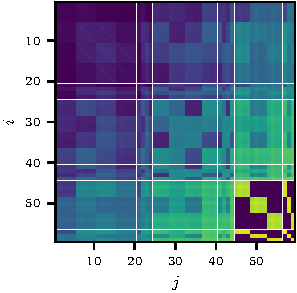
\includegraphics[width=0.8\linewidth]{../kfs/plots/synthetic_rvec_ggn_full.pdf}
  \end{minipage}
  \hfill
  \begin{minipage}[t]{0.485\linewidth}
    \centering
    GGN ($\rvec$)\vspace{1ex}
    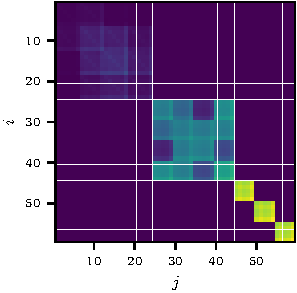
\includegraphics[width=0.8\linewidth]{../kfs/plots/synthetic_rvec_ggn_kfac.pdf}
  \end{minipage}
  \\
  \begin{minipage}[t]{0.485\linewidth}
    \centering
    MC-Fisher ($\rvec$)\vspace{1ex}
    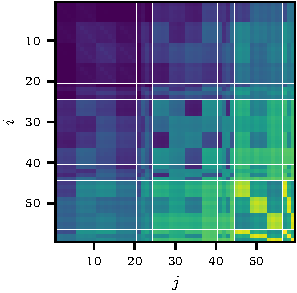
\includegraphics[width=0.8\linewidth]{../kfs/plots/synthetic_rvec_mcfisher_100_full.pdf}
  \end{minipage}
  \hfill
  \begin{minipage}[t]{0.485\linewidth}
    \centering
    MC-Fisher ($\rvec$)\vspace{1ex}
    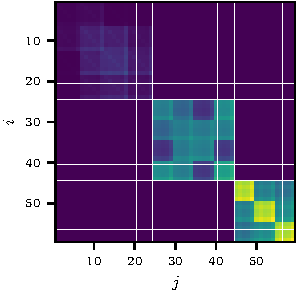
\includegraphics[width=0.8\linewidth]{../kfs/plots/synthetic_rvec_mcfisher_100_kfac.pdf}
  \end{minipage}
  \\
  \begin{minipage}[t]{0.485\linewidth}
    \centering
    Emp-Fisher ($\rvec$)\vspace{1ex}
    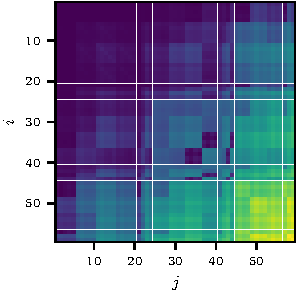
\includegraphics[width=0.8\linewidth]{../kfs/plots/synthetic_rvec_empfisher_full.pdf}
  \end{minipage}
  \hfill
  \begin{minipage}[t]{0.485\linewidth}
    \centering
    Emp-Fisher ($\rvec$)\vspace{1ex}
    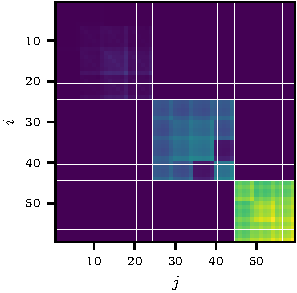
\includegraphics[width=0.8\linewidth]{../kfs/plots/synthetic_rvec_empfisher_kfac.pdf}
  \end{minipage}
  \caption{Visualization of full curvatures (GGN, MC-sampled Fisher and Empirical Fisher) and their corresponding KFAC approximation using $\rvec$-flattening. All curvatures were evaluated on synthetic data ($N = 100$) using an MLP with three fully-connected layers and ReLU activations (5-4-4-3, our notation considers applying the weight matrix and adding the bias as two layers, hence $L=6$) and square loss. For the MC-sampled Fisher we consider $M = 100$ Monte Carlo samples. This follows the setup in \Cref{fig:hessian-block-structure}. For KFAC we concatenate the weight and bias of each layer.
    Plots produced with \repofile{plots/synthetic_kfac}.}
  \label{fig:rvec-kfac-full-comparison}
\end{figure}

\switchcolumn[0]


%%% Local Variables:
%%% mode: latex
%%% TeX-master: "../main"
%%% End:
